%------------------------------------------------------------------------
%  交通流のシミュレーション 
%  The Mathematical Society of Traffic Flow
%  
%  Ver. 1.0 05/12/09  H. Watanabe
%------------------------------------------------------------------------

\documentclass[twocolumn]{jarticle} %二段組の場合
%\documentclass[onecolumn]{jarticle}  %一段組の場合

\usepackage{mstf2}
\usepackage[dvipdfmx]{graphicx}
\usepackage{graphicx}
\usepackage{mathtools}
\graphicspath{{./pic/}}
\usepackage{gensymb}
%------------------------------------------------------------------------

%------------------------------------------------------------------------
%コンパイルコマンド
%1. platex thesis.tex
%2. platex thesis.tex
%3. dvipdfmx thesis.dvi
%4. evince thesis.pdf &
%------------------------------------------------------------------------


\title{%和文タイトル
非線形感覚運動写像ロボットの不完全対面流
一方向走行流への転移と流量のコース幅依存性
}

\titleE{%英文タイトル
Observation of behavior and flow rate by running experiments of multiple robots on elliptical course 
}

\author{%和文氏名
李 方正$^1$, 橋爪 晋平$^2$,本田 泰$^3$
}

\authorE{%英文氏名
Li Fangzheng$^1$, Shimpei Hashizume $^2$,Yasushi Honda $^3$
}

\affiliation{%和文所属
$^1$ 室蘭工業大学大学院 工学研究科 情報電子工学系専攻\\
$^2$ 室蘭工業大学 工学部 情報電子工学系学科\\
$^3$ 室蘭工業大学大学院 しくみ解明系領域
}

\affiliationE{%英文所属
$^1$ Division of Information and Electronic 
Engineering, Graduate School of Engineering, Muroran Institute of Technology, Japan\\
$^2$ Department Information and Electronic 
Engineering,  School of Engineering, Muroran Institute of Technology, Japan\\
$^3$ College of Information and Systems, Muroran Institute of Technology, Japan
}

\abst{%和文概要
本研究では,昆虫や人間の対面走行行為にどんな知能を持っているかを解明するため,ラズパイを基づいてtof距離センサー3つ搭載され,ハイパボリックタンジェント(tanh)関数でセンサーからもらった距離デーダーをロボットの左右モーターの出力に写像して,障害物を避ける走行ロボット開発した.そのロボットを使って,楕円コースで異なる台数のロボットの対面走行実験をして,ロボットの時速,流量と同じ流れになるまでの時間を測定した.
}

\abstE{%英文概要
In this research, in order to unriddle what kinds of intelligence they have in face-to-face moving of insects and humans, we developed wheeled robot which can avoid obstacles based on Raspberry Pi and we use hyperbolic tangent function to transform distance data which got by three laser sensors to of both sides of motors'power output. Then we have done some face-to-face moving experiments with different numbers'robots on ellipical course and we also measured the speed, flow rate and the time spent of robots change to the same direction

}

%------------------------------------------------------------------------
% ここから本文
%------------------------------------------------------------------------

\begin{document}
\maketitle

\section{はじめに}
実世界で,蜂,アリなどの昆虫が簡単な振舞いや匂いで複雑な群れ行為ができる.大きな交差点で,人の密度が高いでも,皆は会話なくて,ぶつからないようにスムーズに対面走行ができる.その中に一体どんな知能が持っている,どのぐらいの知能が必要だと知りたいので,我々は原生生物レベルの感覚と運動直接関連する感覚運動写像での障害物避ける振舞い,反応行動レベルの知能を持つ走行ロボットの対面走行を始めにその知能を解明するである.本稿では,tanh関数を使い非線形感覚運動写像をモデルとし,ラズパイを基づく障害物を避ける走行ロボットを開発した.その走行ロボット(今回,最大8台使われる)を右回りと左回り(変曲点係数bで制御する)の2つグループを分けて楕円コースでの対面走行を実験して,変曲点の係数(b)と初期配置を変化させ,ロボットの振舞いを調査して,ロボットたちの時速,同じ流れになるまでの時間と流量などロボットの基本的な走行情報を測定した.
\section{ロボットの構造}
\subsection{ロボットの身体性}
走行ロボットの正面図と俯瞰図:
\begin{figure}[h]
    \begin{minipage}{0.48\linewidth}
        \centering
        \includegraphics[width=0.9\linewidth]{robot1.jpg}
        \caption{正面図}
    \end{minipage}
    \begin{minipage}{0.48\linewidth}
        \centering
        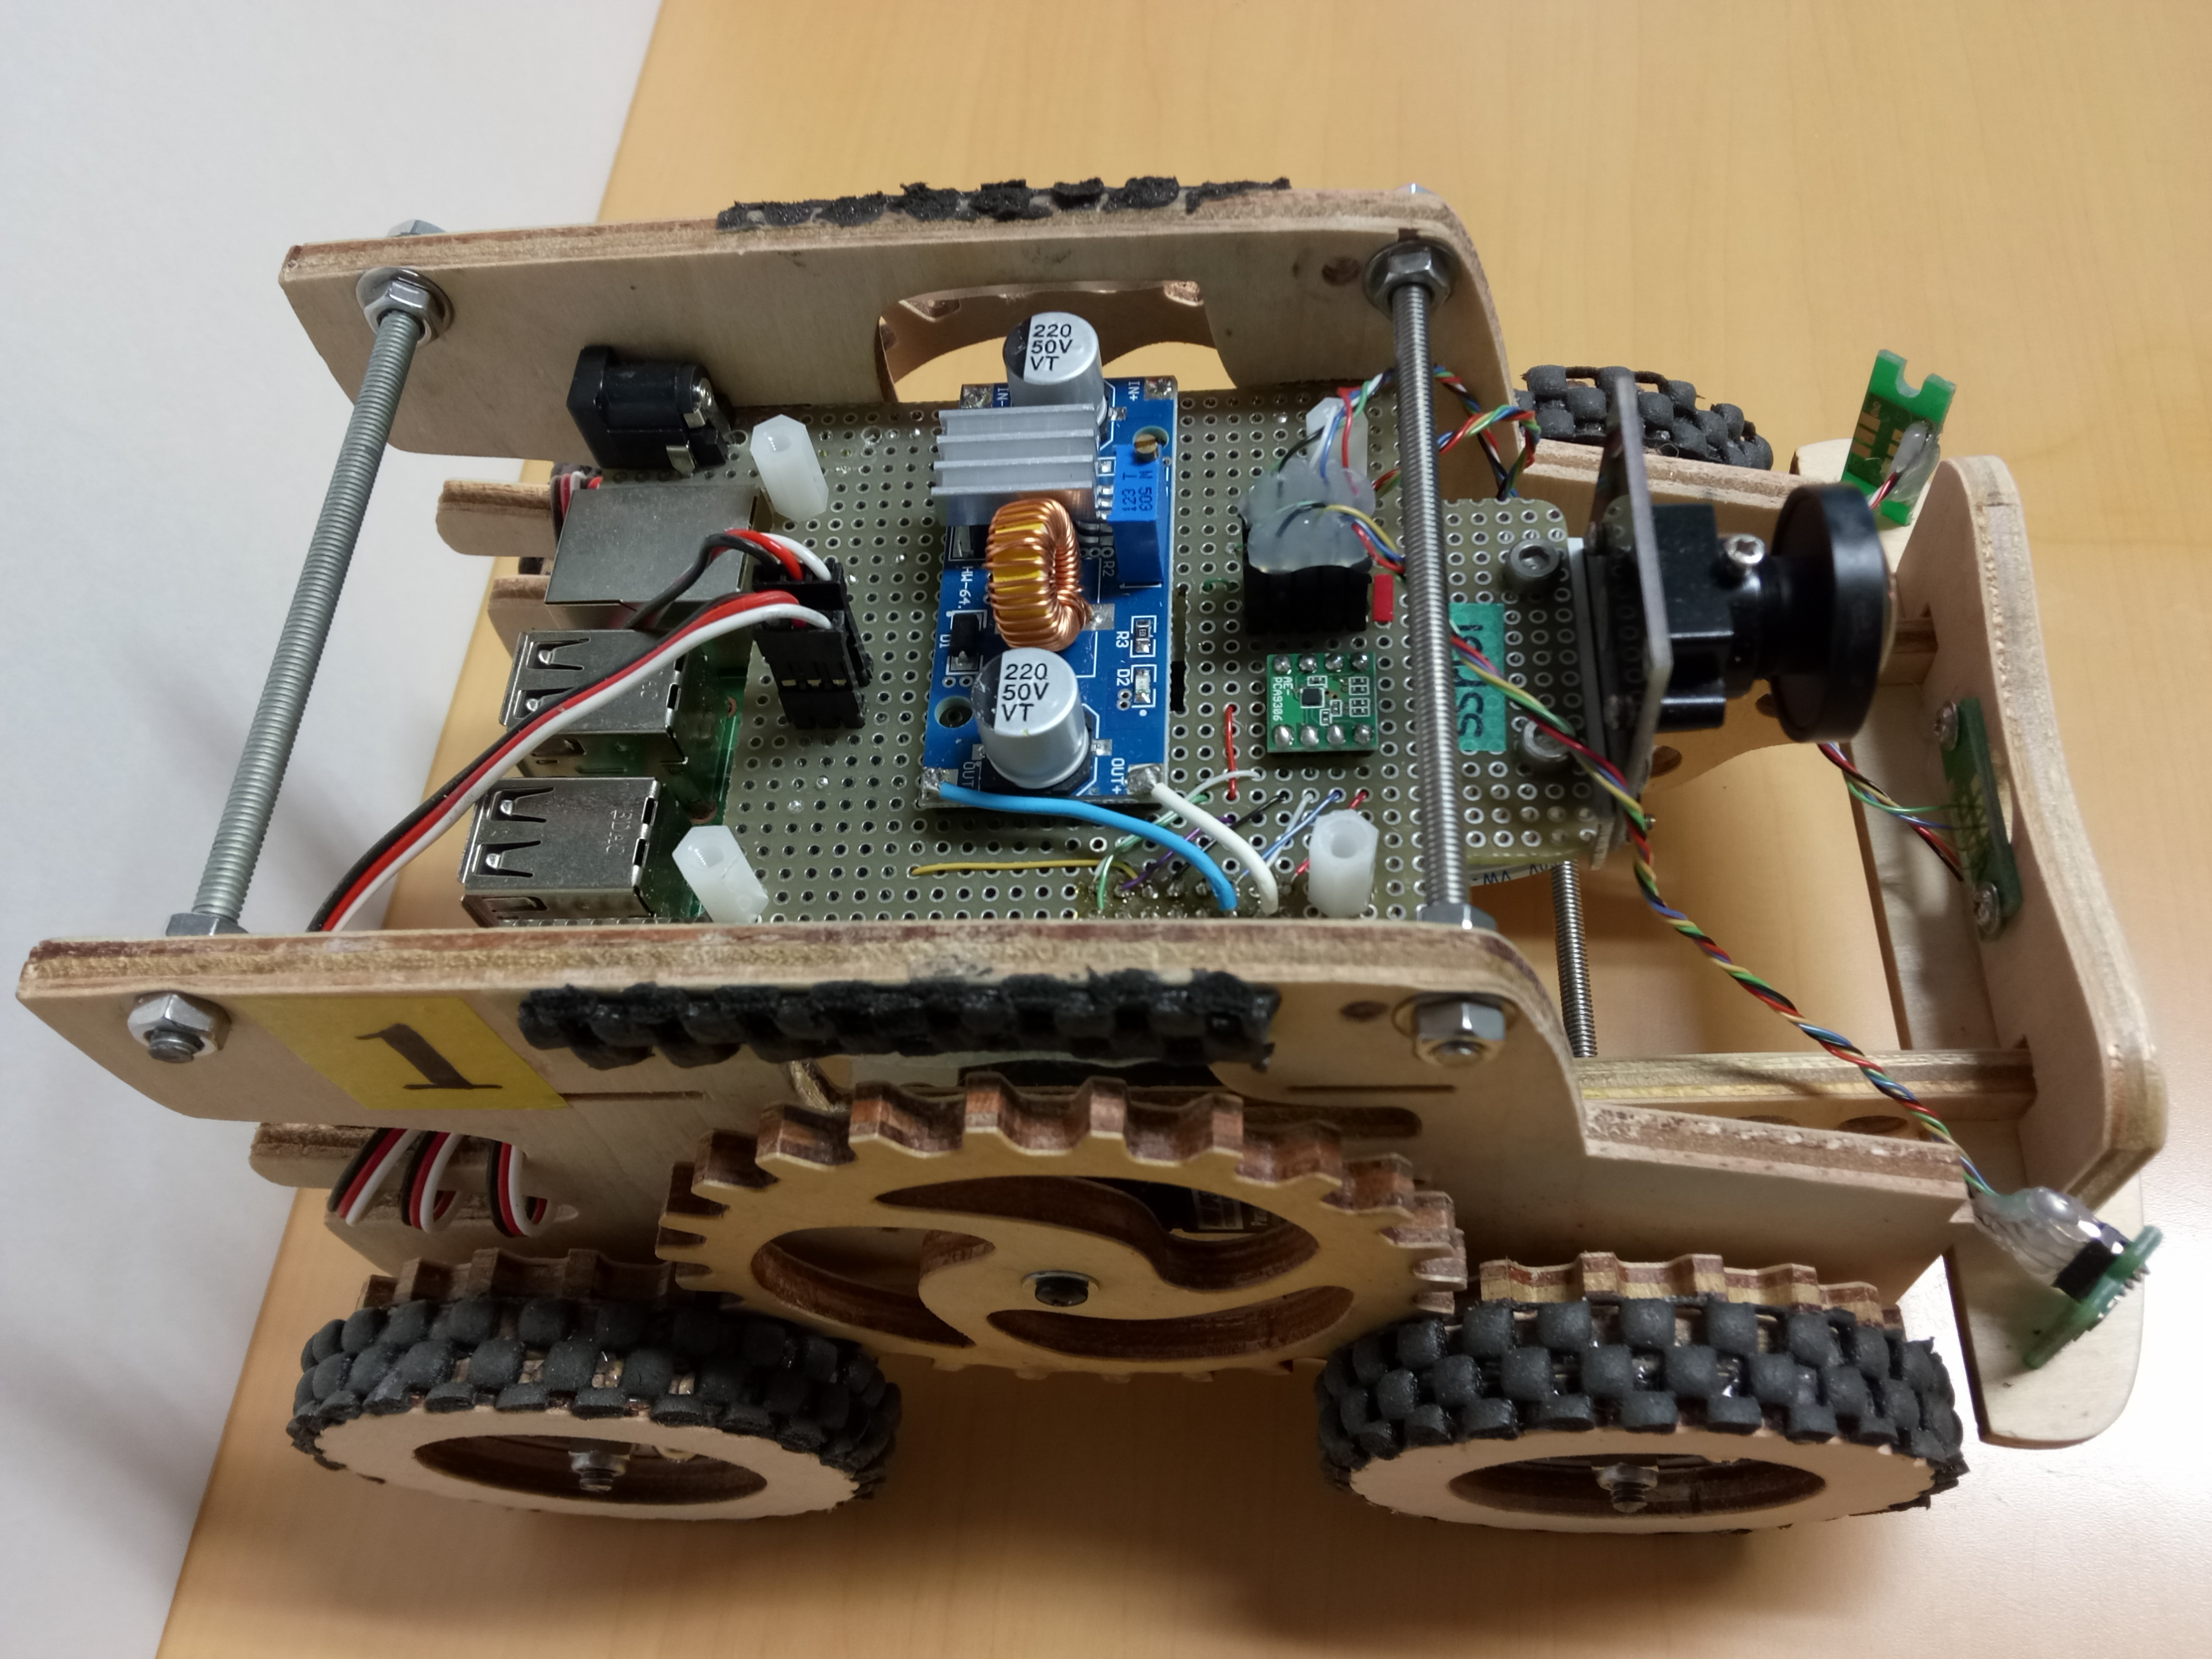
\includegraphics[width=0.9\linewidth]{robot2.jpg}
        \caption{俯瞰図}
    \end{minipage}
\end{figure}
\begin{figure}[h]
        \centering
        \includegraphics[width=1.0\linewidth]{robot4.jpg}
        \caption{左右のセンサー角度表示}
\end{figure}


\begin{table}[htbp]
\begin{center}
\begin{tabular}{|c|c|}
\hline
内容 &  説明 \\
\hline
A & \verb|右の距離センサー| \\
B & \verb|中央の距離センサー| \\
C & \verb|左の距離センサー| \\
D & \verb|カメラ(使っていない)| \\
E & \verb|右モーター| \\
F & \verb|左モーター| \\
制御システム & \verb|ラズパイ| \\
左右センサー角度 & \verb|45|\degree \\
\hline
\end{tabular}
\end{center}
\caption{
ロボットの説明
}
\end{table}
今回使っているのは4輪木造走行ロボットである,人間や昆虫の走行特徴に近似するため,左右の車輪は左右のモーターで独自に制御して,超信地旋回できるようになる.tof距離センサーが赤外線の反射で距離を測るので,超音波より測る範囲が狭いけど,体積が小さく,精度が高くて,複数ロボットの場合,ロボット同士間の妨害も減少できる.

\subsection{感覚運動写像モデル}

感覚運動写像とは,センサー値を変数とする関数によってモーターの出力を決定することであり,その瞬間のセンサー値だけを使うと,最も単純な反応行動のための知能の一つである.
本研究では,非線形写像モデルが使われている.

1.距離デーダーの相乗平均:

\begin{equation}
  x_L = e^{\gamma \ln d_C} \cdot e^{(1-\gamma)\ln d_L} 
\end{equation}
\begin{equation}
  x_R = e^{\gamma \ln d_C} \cdot e^{(1-\gamma)\ln d_R} 
\end{equation}

中央のセンサーでもらった距離デーダー($d_C$)と左のセンサーでもらった距離デーダー($d_L$)が式(1)で計算して,左の感覚運動写像方程式の入力($x_L$)がもらえる,同じように,真中のセンサーでもらった距離デーダー($d_R$)と右のセンサーでもらった距離デーダー($d_R$)が式(2)で計算して,右の感覚運動写像の入力($x_R$)がもらえる.$\gamma$は重みであり,$\gamma$イコール0.33のとき,等加重である.

2.感覚運動写像:
\begin{equation}
\begin{aligned}
  m_{\rm R} = &\alpha_{1{\rm L}} \rm tanh(\beta_{1{\rm L}}(x_{\rm L} - b_{\rm L})) + \\
        &\alpha_{2{\rm L}} \rm tanh(\beta_2{\rm L}(x_{\rm L} - b_{\rm L})) + c_L
\end{aligned}
\end{equation}

\begin{equation}
\begin{aligned}
  m_L = &\alpha_{1{\rm R}}tanh(\beta_{1{\rm R}}(x_{\rm R} - b_{\rm R})) + \\
        &\alpha_{2{\rm R}}tanh(\beta_{2{\rm R}}(x_{\rm R} - b_{\rm R})) + c_{\rm R}
\end{aligned}
\end{equation}
式(1)と(2)でもらった$x_L$と$x_R$を式(3)と(4)に代入して,ロボットの右モーターの出力($f_R$)と左モーターの出力($f_L$)が計算できる.係数$\alpha$がロボットの最大速度を制御する,係数$\beta$がtanhの傾きを制御する,係数$b$が関数の変曲点の位置を制御する,係数$c$が関数のだて軸上の位置を制御する. 



\section{走行実験}
直線と円形両方あり,一回じゃなくて,ぐるぐる回って複数の対面走行できるように,楕円コースで実験する.コースの中にロボットをランダムに配置して速度0からほぼ同時にスタート,約8分間実験する.ロボットたちがtof距離センサーでコースの壁までの距離を測って,感覚運動写像により走行する.半分のロボットが右回り($b_L>b_R$),残りのロボットが左回り($b_L<b_R$).図の赤い線がスタートとし,ロボットが左から右へ線を越えたら流量+1,右から左へ線を越えたら流量-1

\begin{figure}[htb]
\centering
\includegraphics[width=0.5\linewidth]{course1.jpg}
\includegraphics[width=0.5\linewidth]{pic/Oval.eps}
\caption{
コース
}
\label{fig_dummy}
\end{figure}


\begin{table}[!htb]
\begin{center}
\begin{tabular}{|cl|}
\hline
内容 &  数値\\
\hline
コース幅 & \verb|56|($mm$) \\
コース長さ & \verb|7.32|($m$) \\
コース面積 & \verb|4.053|($m^2$) \\
ロボット幅 & \verb|13.5|($mm$) \\
ロボット長さ & \verb|20.2|($mm$) \\
ロボット高さ & \verb|12.2|($mm$) \\
\hline
\end{tabular}
\end{center}
\caption{
コース参数とロボット参数
}
\end{table}


\begin{table}[!htb]
\begin{center}
\begin{tabular}{|c|c|c|c|c|c|c|}
\hline
係数 & $\alpha_{1L}$ & $\alpha_{2L}$ & $\beta_{1L}$ & $\beta_{2L}$ & $c_L$ \\
\hline
値 & \verb|30| & \verb|30| & \verb|0.004| & \verb|10| & \verb|0| \\
\hline
係数 & $\alpha_{1R}$ & $\alpha_{2R}$ & $\beta_{1R}$ & $\beta_{2R}$ & $c_R$ \\
\hline
値 & \verb|30|& \verb|30| & \verb|0.004| & \verb|10| & \verb|0| \\
\hline
\end{tabular}
\end{center}
\end{table}

\begin{table}[!htb]
\begin{center}
\begin{tabular}{|c|c|}
\hline
 奇数番号ロボット$b_L$ & 偶数番号ロボット$b_R$ \\
\hline
 160 & 260 \\
\hline
 奇数番号ロボット$b_R$ & 偶数番号ロボット$b_R$ \\
\hline
 260 & 160 \\
\hline
\end{tabular}
\end{center}
\caption{
パラメーターの設定
}
\end{table}


\section{実験結果}
\subsection{記録内容の説明}

\begin{enumerate}
\item $b_L>b_R$:ロボットが右曲がり易い
\item $b_L<b_R$:ロボットが左曲がり易い
\item 初期配置:ロボットの位置はランダムで,向きを変化する(奇左偶右:奇数番号のロボットが最初左回りの方向に置く,偶数番号のロボットが最初右回りの方向に置く)
%\item 密度:ロボット台数/コース面積
\item $T_{\rm sd}$:全てのロボットのスタートから全てのロボットが一方向走行するまでの所要時間
\item 渋滞時間割合:$T_{\rm sd}$に対して,渋滞時間の割合
\item 同じ流れ方向:同じ流れになる時間後の
          同一方向走行の方向
\item 流量:コースの計測線を通過したロボットの数
  (左から右へ通過は流量+1,逆たら流量-1)
\end{enumerate}

\subsection{時速の測定}
ロボットが一つずつ5周回って,時速を計算する
\begin{table}[!ht]
\begin{center}
\begin{tabular}{|c|l|r|}
\hline
ロボット番号 &  5周タイム & 時速 \\
\hline
101 & \verb|3分31秒|  &  \verb|713.64|$m/h$ \\
102 & \verb|2分36秒|  &  \verb|835.61|$m/h$ \\
103 & \verb|2分43秒|  &  \verb|802.85|$m/h$ \\
104 & \verb|2分36秒|  &  \verb|836.68|$m/h$ \\
105 & \verb|2分31秒|  &  \verb|863.14|$m/h$ \\
106 & \verb|2分52秒|  &  \verb|761.33|$m/h$ \\
107 & \verb|2分59秒|  &  \verb|729.1|$m/h$ \\
108 & \verb|2分52秒|  &  \verb|757.81|$m/h$ \\
\hline
\end{tabular}
\end{center}
\caption{
ロボットの時速
}
\end{table}


\subsection{幅による流量の測定}

\begin{table}[!ht]
\begin{center}
\begin{tabular}{|c|c|c|c|c|}
\hline
初期配置 & 同方向時間 & 流量 & 渋滞時間 \\
\hline
奇右偶左 & 480秒 & -1 & 83% \\
\hline
奇左偶右 & 480秒 & 2 & 88% \\
\hline
\end{tabular}
\end{center}
\caption{
幅:43cm
}
\end{table}

\begin{table}[!ht]
\begin{center}
\begin{tabular}{|c|c|c|c|c|}
\hline
初期配置 & 同方向時間 & 流量 & 渋滞時間 \\
\hline
奇右偶左 & 426秒 & -15 & 36% \\
\hline
奇左偶右 & 480秒 & -8 & 45% \\
\hline
\end{tabular}
\end{center}
\caption{
幅:49.5cm
}
\end{table}

\begin{table}[!ht]
\begin{center}
\begin{tabular}{|c|c|c|c|c|}
\hline
初期配置 & 同方向時間 & 流量 & 渋滞時間 \\
\hline
奇右偶左 & 135秒 & 14 & 7% \\
\hline
奇左偶右 & 230秒 & -8 & 29% \\
\hline
\end{tabular}
\end{center}
\caption{
幅:56cm
}
\end{table}

\begin{table}[!ht]
\begin{center}
\begin{tabular}{|c|c|c|c|c|}
\hline
初期配置 & 同方向時間 & 流量 & 渋滞時間 \\
\hline
奇右偶左 & 85秒 & -12 & 0 \\
\hline
奇左偶右 & 243秒 & -3 & 4% \\
\hline
\end{tabular}
\end{center}
\caption{
幅:62.5cm
}
\end{table}

\begin{table}[!ht]
\begin{center}
\begin{tabular}{|c|c|c|c|c|}
\hline
初期配置 & 同方向時間 & 流量 & 渋滞時間 \\
\hline
奇右偶左 & 78秒 & -6 & 0 \\
\hline
奇左偶右 & 237秒 & 16 & 0 \\
\hline
\end{tabular}
\end{center}
\caption{
幅:69cm
}
\end{table}

\end{document}


